
\section{Making Modeling Choices}
\label{sec:modeling-choices}

\subsection{Computational box} \label{subsect:coords} PISM does all simulations in a computational box\index{PISM!computational box} which is rectangular in the PISM coordinates.

The coordinate system has horizontal coordinates $x,y$ and a vertical coordinate $z$.  The $z$ coordinate is measured positive upward from the base of the ice and it is exactly opposite to the vector of gravity.  The surface $z=0$ is the base of the ice, however, and thus is usually not horizontal in the sense of being parallel to the geoid.   The surface $z=0$ is the base of the ice both when the ice is grounded and when the ice is floating.

Bed topography is, of course, allowed.  In fact, when the ice is grounded, the true physical vertical coordinate $z'$, namely the coordinate measure relative to a reference geoid, is given by $z'=z+b(x,y)$ where $b(x,y)$ is the bed topography.  The surface $z'=h(x,y)$ is the surface of the ice.

In the grounded case the equation $h(x,y)=H(x,y)+b(x,y)$ always applies if $H(x,y)$ is the thickness of the ice.  In the floating case, the physical vertical coordinate is $z'=z-(\rho_i/\rho_s) H(x,y)$ where $\rho_i$ is the density of ice and $\rho_s$ the density of sea water.  Again $z=0$ is the base of the ice, which is the surface $z' = -(\rho_i/\rho_s) H(x,y)$.  The surface of the ice is $h(x,y) = (1-\rho_i/\rho_s) H(x,y)$.  All we know about the bed elevations is that they are below the base of the ice when the ice is floating.  That is, the \emph{floatation criterion} $-(\rho_i/\rho_s) H(x,y) > b(x,y)$ applies.

The computational box can extend downward into the bedrock.  As $z=0$ is the base of the ice, the bedrock corresponds to negative $z$ values regardless of the sign of its true (i.e.~$z'$) elevation.

The extent of the computational box, along with its bedrock extension downward, is determined by four numbers \t{Lx}, \t{Ly}, \t{Lz}, and \t{Lbz}.  The first two of these are half-widths and have units of kilometers when set by options or displayed.  The extent of the computational box for the ice is directly controlled by the options \intextoption{Lx}, \intextoption{Ly}, and \intextoption{Lz} as described in Appendix \ref{sect:options}.  In particular, \t{-Lx} and \t{-Ly} options should include values in kilometers while \t{-Lz} and \t{-Lbz} should be in meters. See Figure \ref{fig:rectilinearbox}.

\begin{figure}[ht]
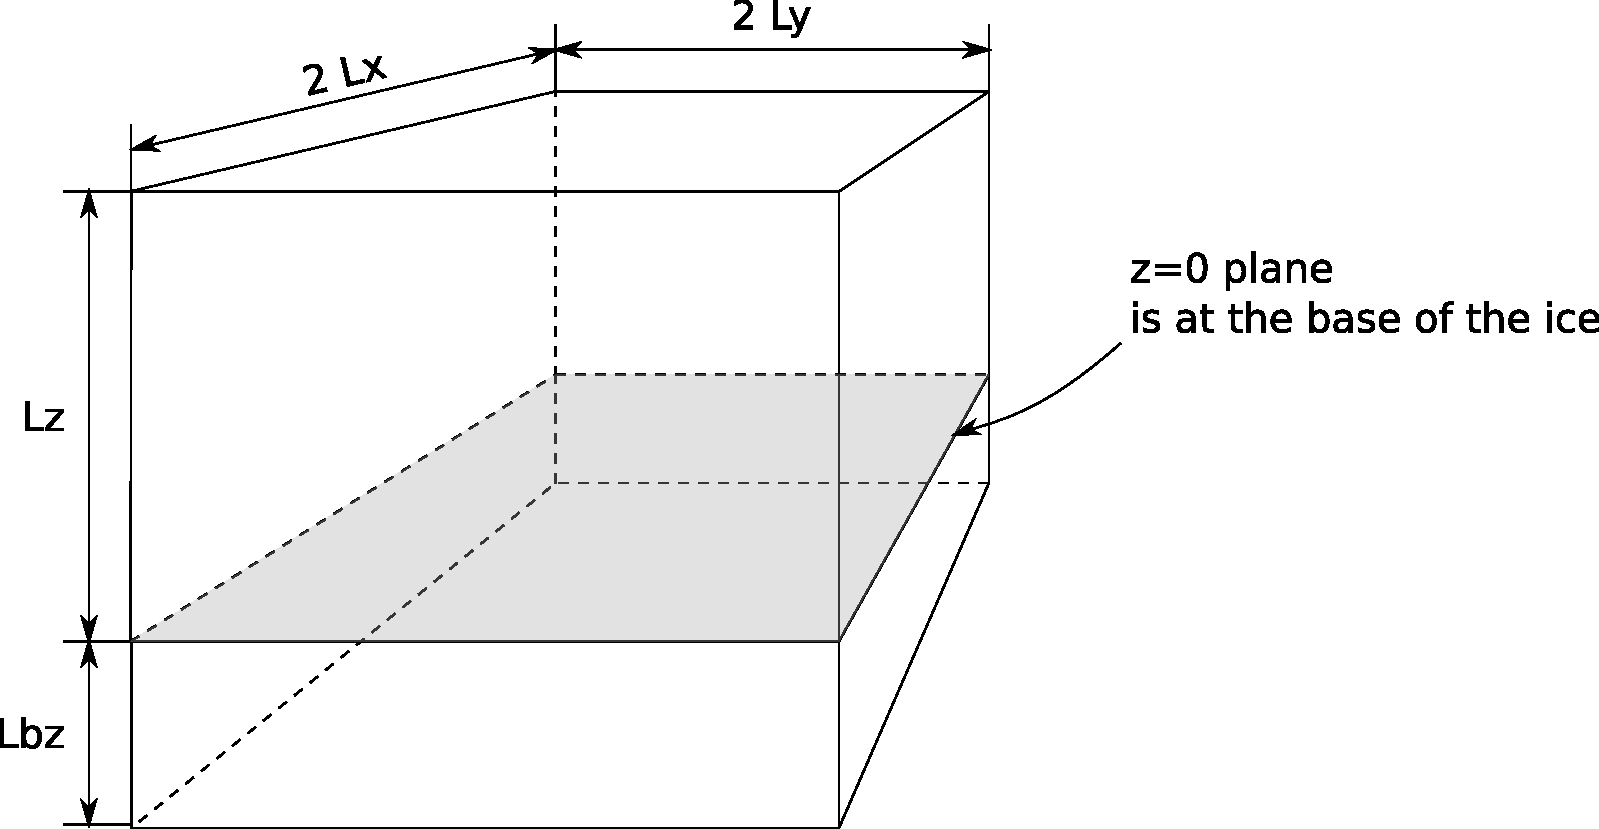
\includegraphics[width=4.0in,keepaspectratio=true]{rectilinearbox}
\caption{PISM's computational box.}
\label{fig:rectilinearbox}
\end{figure}


\subsection{Grid}
\label{subsect:grid}
The PISM grid\index{PISM!grid} covering the computational box is equally spaced in horizontal ($x$ and $y$) directions.  Vertical spacing is quadratic by default (see below) but optionally a different spacing scheme can be chosen.  (Choose with options \intextoption{z\und spacing} and \intextoption{zb\und spacing}.)

The grid is described by four numbers, namely the number of grid points \verb|Mx| in the $x$ direction, the number \verb|My| in the $y$ direction, the number \verb|Mz| in the $z$ direction within the ice, and the number \verb|Mbz| in the $z$ direction within the bedrock thermal layer.  These are specified by options \intextoption{Mx}, \intextoption{My}, \intextoption{Mz}, and \intextoption{Mbz}, respectively, as in Appendix \ref{sect:options}.  The defaults are 61, 61, 31, and 1, respectively.

Note that \verb|Mx|, \verb|My|, \verb|Mz|, and \verb|Mbz| all indicate the number of grid \emph{points}.  The number of grid \emph{spaces} are one less, thus 60, 60, 30, and 0 in the default case.  The lowest grid point in a column of ice, at $z=0$, coincides with the highest grid point in the bedrock, so \verb|Mbz| must always be at least one.

Default spacing is a quadratic function: the spacing is smaller near the base than near the top. (See the documentation of \verb|IceGrid::compute_ice_vertical_levels()| in PISM's class browser for more info and formulas defining the spacing.)

When a thermal bedrock layer is used, the distance \t{Lbz} is controlled by the \intextoption{Lbz} option.

If one initializes PISM from a saved model state using \intextoption{i} then the input model state controls the parameters \t{Mx}, \t{My}, \t{Mz}, and \t{Mbz}.  For instance, the command

\verb|$  pismr -i foo.nc -y 100|

\noindent should work fine if \verb|foo.nc| was a valid PISM model file.  The command

\verb|$  pismr -i foo.nc -Mz 201 -y 100|

\noindent will give a warning that ``\verb|PISM WARNING: ignoring command-line option '-Mz'|'' because \verb|-i| input files take precedence.

Otherwise, one is allowed to specify the grid when PISM is started.  In particular, the user should specify the grid when using \intextoption{boot\und from} or when initializing a simplified geometry experiment or a verification test, though defaults are generally present in these cases.  See sections \ref{sect:start} and \ref{sect:boot} for examples and explanation.


\subsection{Diagnostic computations}  As a diagnostic example, using the EISMINT II final state computed in section \ref{sect:start}, try\index{pismd}

\verb|pismd -i eisIIA200k.nc -o eisIIA200k_diag.nc|

\noindent The result is a NetCDF file \verb|eisIIA200k_diag.nc| which contains the full three-dimensional velocity field in the scalar NetCDF variables \verb|uvel|, \verb|vvel|, and \verb|wvel|.

The velocity field saved by \verb|pismd| is the one which would be computed at the \emph{next} time step in an evolution run.  That is, if we also run\index{pisms}

\verb|pisms -eisII A -i eisIIA200k.nc -y 0 -o eisIIA200k_plus.nc|

\noindent then the horizontal velocity field computed in this single time step run is the same as that saved in \verb|eisIIA200k_diag.nc|.\footnote{For this example, one can use a NetCDF Operator\index{NCO (NetCDF Operators)!ncdiff} to check that the two saved NetCDF files contain the same vertically-averaged horizontal velocity field; just do \t{ncdiff -v cbar} \dots}

This diagnostic mode is most frequently associated to the modeling of ice shelves and ice streams.  Subsection \ref{sect:ross} describes using \verb|pismd| to model the Ross ice shelf \cite{MacAyealetal}.  Verification tests I and J, section \ref{sect:verif}, are diagnostic calculations using the SSA.

Note that the NetCDF model state saved by PISM at the end of an \emph{evolution} run does not, by default, contain the three-dimensional velocity field.  Instead, it contains just the variables which are needed to restart the run, especially the ice geometry and temperature field.  One can also force PISM to save the full velocity field at the end of a time-stepping run using the option \intextoption{f3d}.  The diagnostic executable \verb|pismd| saves the full three-dimensional velocity field by default.  Either way, saving the full velocity field roughly doubles the size of the saved NetCDF file.



\subsection{Computing ice age} \label{subsect:age} By default, PISM does not compute the age of the ice\index{PISM!modeling the age of the ice} because it does not directly impact ice flow using the default flow laws.   It is very easy to turn on.  Just set \intextoption{age}.


\subsection{Positive degree-day model}  \label{subsect:pdd} \index{positive degree day model} \index{PDD (positive degree day model)} \index{PISM!default positive degree day model}  The default atmospheric climate assumption made by the \verb|pismr| and \verb|pgrn| executables is that the input file will supply surface mass balance and ice surface temperature in variables \verb|acab| and \verb|artm|, respectively.  The supplied surface mass balance \verb|acab| is assumed to be the net surface balance, which is not the snow accumulation rate when melting can occur, and it must be in units of ice-equivalent thickness per time.  The supplied surface temperature \verb|artm| is regarded as the mean annual surface temperature, at a point in the ice below the completion of firn processes \cite{Hock05}.  The mass conservation equation for the ice sheet requires the surface mass balance, while the conservation of energy model requires the ice surface temperature as a boundary condition.

These assumptions about supplied climate are not very realistic for practical glaciological observations.  If the input data actually includes the annual snow-fall accumulation then one might want to compute the surface mass balance according to some model of how much of the snow is transformed to ice, and how much ablates or is transported away, using a modeled time- and space-dependent temperature.  An example of such a model is a \emph{positive degree day} model \cite{Hock05}, a ``PDD''.  The default PDD used by PISM, turned on by option \intextoption{-surface pdd}, comes from the EISMINT-Greenland intercomparison (section \ref{sect:green} and \cite{RitzEISMINT}), but it has controllable parameters.

The snow accumulation rate data should be supplied to this PDD in the input variable \verb|snowprecip|, and should already be measured in ice-equivalent thickness per time (e.g.~\verb|m s-1|).  The annual mean snow temperature is again the variable \verb|artm| and should have units K.

There are parameters controlling the seasonal temperature cycle.  The positive difference between the peak of seasonal temperatures and the mean (average) is called the ``summer warming.''  The default temperature cycle has a constant amount of summer warming, controlled by option \intextoption{pdd\und summer\und warming}.  By default the peak of the seasonal cycle occurs on August 1, Julian day 243 (option \intextoption{pdd\und summer\und peak\und day} can override this).  The annual mean temperature is grid-point dependent, specified by the input surface temperature map in variable \verb|artm|, but the timing of the peak and the amount of summer warming are applied equally everywhere.

A PDD generally adds ``white noise'' to the seasonal cycle to simulate additional daily variability associated to the vagaries of weather.  This additional random variation is quite significant, as the seasonal cycle may never reach the melting point but that point may be reached with some probability, in the presence of the daily variability, and thus melt may occur.  Concretely, a normally-distributed, mean zero random temperature increment is added to the seasonal cycle.  The standard deviation of the daily variability is controlled by \intextoption{pdd\und std\und dev}, and defaults to 5 degrees.  There is no particular assumed spatial correlation of daily variability.

The number of positive degree days is computed as the magnitude of the temperature excursion above $0\!\phantom{|}^\circ \text{C}$ multiplied by the duration (in days) when it is above zero.  In PISM there are actually two methods for computing the number of positive degree days.  The first computes only the expected value, by the method described in \cite{CalovGreve05}.  This is the default when a PDD is chosen (i.e.~option \intextoption{pdd}).  The second is a monte carlo simulation of the white noise itself, chosen by \intextoption{pdd\und rand}.  This monte carlo simulation adds the same daily variation at every point, though the seasonal cycle is (generally) location dependent.  If repeatable randomness is desired use \intextoption{pdd\und repeatable} instead of \verb|-pdd_rand|.

The number of positive degree days is multiplied by a coefficient (\intextoption{pdd\und factor\und snow}) to compute the amount of snow melted.  Of the melted snow, a fraction (\intextoption{pdd\und refreeze}) is kept as ice.  This ice, plus all unmelted snow (already measured as ice-equivalent) is added to the mass balance, unless the number of positive degree days exceeds that required to melt all of the snow.  In this latter case, in which there are excess positive degree days available for melting, the excess is multiplied by a coefficient (\intextoption{pdd\und factor\und ice}) to compute how much ice is melted.  In this case actual ablation occurs at that location.

There is an executable for testing the PDD model without invoking ice dynamics, namely \verb|pcctest|.  See subsection \ref{subsect:pcctest}.  Section \ref{sect:green} demonstrates the PDD model and \verb|pcctest|.


\subsection{Floatation criterion and mask} \label{subsect:floatmask}  The most basic decision about ice dynamics made internally by PISM is whether to apply the ``floatation criterion'' to determine whether the ice is floating on the ocean or not.  In an evolution run this decision is made at each time step and the result is stored in the \t{mask}.

The possible values of the \t{mask}\index{mask} are given in Table \ref{tab:maskvals}.  The mask does not by itself determine ice dynamics.  For instance, when ice is floating (either value \verb|MASK_FLOATING| or \verb|MASK_FLOATING_OCEAN0|) the usual choice for ice dynamics is SSA, but the user can choose not to apply that model by leaving off the option \verb|-ssa|.

\begin{table}[ht]
\caption{The PISM mask\index{mask}, in combination with user options, determines the dynamical model.}\label{tab:maskvals} 
\small
\begin{tabular}{p{0.25\linewidth}p{0.65\linewidth}}\hline
\textbf{Mask value} & \textbf{Meaning}\\ \hline
1=\verb|SHEET| & ice is grounded (and only the SIA is always applied) \\
2=\verb|DRAGGING| & ice is grounded (and the SSA is applied if option \verb|-ssa| is given) \\
3=\verb|FLOATING| & ice is floating (and the SSA is applied if option \verb|-ssa| is given) \\
7=\verb|FLOATING_OCEAN0| & same as \verb|FLOATING|, but the grid point was ice free ocean at initialization of the model by \verb|-boot_from|; ice with this value will calve off if option \verb|-ocean_kill| is given.\\
\hline\end{tabular}
\normalsize
\end{table}

Assuming the geometry of the ice evolves (which can be turned off by option \intextoption{no\und mass}), and assuming an ocean exists (which can be turned off by option \intextoption{dry}), then at each time step the mask can change.  Ice which becomes floating is marked as \verb|FLOATING| while ice which becomes grounded is either marked as \verb|SHEET| or \verb|DRAGGING|.  The decision between \verb|SHEET| or \verb|DRAGGING| is made by a vote-by-neighbors scheme in the most general case.  When both \intextoption{ssa} and \intextoption{super} are given all grounded ice is \verb|DRAGGING|, however.

\subsection{Plastic till free boundary problem for ice streams; SSA as a sliding law}  \label{subsect:plastic}
WARNING: The models described in this subsection are still under active development, and thus we give only a sketch.

The shallow shelf approximation (SSA)\index{SSA (shallow shelf approximation)} stress balance is used in PISM to describe the sliding of grounded ice and the formation of ice streams \cite{BBssasliding}, as well as being used as the only stress balance for floating ice.  For the SSA with ``plastic'' or ``Coulomb'' till the locations of ice streams is determined as part of a free boundary problem \cite{SchoofStream}.  We believe that this mathematical description of ice streams, by Schoof, should be regarded as the best known ``sliding law'' for the SIA \cite{BBssasliding}.\index{SIA (shallow ice approximation)!sliding law}

Schoof's model \cite{SchoofStream} describes emergent ice streams within a larger ice sheet and ice shelf system.  It explains the existence of ice streams by a combination of the plastic failure of the till and the SSA approximation of the balance of momentum.  

In PISM the user gives the options \verb|-ssa -plastic -super| to turn on the use of the plastic till SSA as a sliding law.  All grounded points are immediately marked as SSA (i.e.~as \verb|DRAGGING|).  At these points a yield stress is computed from the amount of stored basal water and from a (generally) spatially-varying till strength, \verb|tillphi| in an input or output file.  The amount of stored basal water is thermodynamically determined.

\begin{table}[ht]
\caption{Using the SSA stress balance in PISM.}\label{tab:ssausage} 
\small
\begin{tabular}{p{0.25\linewidth}p{0.65\linewidth}}\hline
\textbf{Option combination} & \textbf{Meaning}\\ \hline
\intextoption{ssa} & Floating ice uses SSA, and at all points marked \t{DRAGGING}. Basal resistance for grounded ice is plastic (see \intextoption{pseudo\und plastic} to control parameters) but uses fixed field \t{tauc} with no update. \\
\t{-ssa} \intextoption{plastic} & As above, but all grounded points are forced to be \t{DRAGGING} and \t{tauc} is updated at each time step using stored map \t{tillphi} and evolving basal melt water effective thickness \t{bwat}. \\
\t{-ssa -plastic} \intextoption{super} & The recommended default sliding law.  Combines SSA-computed velocity, using plastic till, with SIA-computed velocity as in \cite{BBssasliding}. \\
\hline\end{tabular}
\normalsize
\end{table}

The basal resistance is actually determined by a controllable ``pseudo-plastic'' model.  Specifically, stress is a generally a power law function of basal sliding velocity $\mathbf{u}$:
   $$\tau_b = \tau_c \frac{|\mathbf{u}|^{q-1}}{u_{\text{threshold}}^q}\, \mathbf{u}.$$
Here $\tau_c$ corresponds to the variable \verb|tauc| in PISM input and output files, $q$ is the power controlled by \intextoption{pseudo\und plastic\und q}, and the threshold velocity $u_{\text{threshold}}$ is controlled by \intextoption{pseudo\und plastic\und uthreshold}.  The purely plastic case is $q=0$---see \cite{SchoofStream} for precise interpretation---and the linear case is $q=1$, in which case the coefficient of velocity, $\tau_c/u_{\text{threshold}}$, is more commonly called $\beta$ or $\beta^2$ \cite{MacAyeal}.

In our model the till yield stress $\tau_c$ necessarily represents the strength of the aggregate material at the base of an ice sheet, a poorly observed mixture of liquid water, ice, and granular till.  The value of $\tau_c$ is determined by a basal water model:
\begin{equation*}
   \tau_c = (\tan\phi)\,(\rho g H - p_w).
\end{equation*}
\cite[Chapter 8]{Paterson}.  Here $H$ is the ice thickness, $\rho$ the ice density, $g$ the acceleration of gravity, $p_w$ is the modeled pore water pressure, and $\phi$ is the till friction angle \verb|tillphi|.  The difference $(\rho g H - p_w)$ is the modeled value of the effective pressure on the material till.  Option \intextoption{plastic\und pwfrac} controls how $p_w$ is determined from the effective thickness of basal water, the quantity in \verb|bwat|.

The scripts in \t{examples/pst} perform the experiments described in \cite{BBssasliding}, and represent the most thorough test of these mechanisms.

Test I in the verification suite\index{verification tests} uses an exact solution to the Schoof model, that is, the model described by \t{-ssa -plastic}.

In the \t{-ssa -plastic -super} case especially, the determination of basal resistance comes from a stored basal till material property \verb|tillphi|, the till friction angle.  We find that an effective way to determine \verb|tillphi| is to make it a function of bed elevation.  Option \intextoption{topg\und to\und till} does this.

\subsection{Earth deformation models} \label{subsect:beddef} \index{earth deformation} \index{PISM!earth deformation models, using}   Options
\intextoption{bed\und def\und iso} and \intextoption{bed\und def\und lc} turn on bed deformation models.  The former uses the very minimal assumption of instantaneous pointwise (i.e.~independently at each point in the map plan) isostatic adjustment.  

The latter is much more effective.  It is based on papers by Lingle and Clark \cite{LingleClark}\index{Lingle, Craig} \index{Clark, J.} and \cite{BLKfastearth}.  It is essentially instantaneous computationally because of use of the Fast Fourier Transform to solve the relevant differential equation.  Among other practical features, the rate of bed movement (uplift) is stored in the PISM output file and then is used to initialize the next part of the run.  If observed uplift data is available, it can be used along with \intextoption{boot\und from} to initialize the model so that it starts with the given uplift rate.

Example runs to compare these models are
\begin{verbatim}
$ mpiexec -n 4 pisms -eisII A -z_spacing quadratic -y 8000 -o eisIIA_nobd.nc
$ mpiexec -n 4 pisms -eisII A -z_spacing quadratic -bed_def_iso -y 8000 -o eisIIA_bdiso.nc
$ mpiexec -n 4 pisms -eisII A -z_spacing quadratic -bed_def_lc -y 8000 -o eisIIA_bdlc.nc
\end{verbatim}
Compare the \verb|topg|, \verb|usurf|, and \verb|dbdt| variables in the resulting output files.

Test H in section \ref{sect:verif} can be used to reproduce the comparison done in \cite{BLKfastearth}.

